%\section[Gas \Cherenkov{} Counters]{Gas \Cherenkov{} Counters
\chapter[Gas \Cherenkov{} Counters]{Gas \Cherenkov{} Counters
\footnote{
  $CVS~revision~ $Id: gas-cer.tex,v 1.4 2003/12/13 06:23:38 gen Exp $ $
}
\footnote{Author: B. B. Wojtsekhowski \email{bogdanw@jlab.org}}
}

A gas \Cherenkov{} detector filled  with CO$_{2}$ at atmospheric 
pressure is mounted between the trigger scintillator planes S1 and S2. 
The detector allows an electron identification
with 99\% efficiency and has a threshold for pions at 4.8 GeV/$c$.
The detector has ten spherical mirrors with 80 cm focal length, each
viewed by a PMT (Burle 8854);
the light-weight mirrors were developed at INFN.
The focusing of the \Cherenkov{} ring onto a
small area of the PMT photo-cathode leads to a high current density  near
the anode. To prevent a non-linear PMT response even in the case of few
photoelectrons requires a progressive HV divider.
The length of the particle path in the gas radiator is 130 cm for the gas
\Cherenkov{} in the HRS-R, leading to an average of about twelve photoelectrons.
In the HRS-L, the gas \Cherenkov{} detector in its standard configuration has
a path length of 80~cm, yielding seven photoelectrons on average.
The total amount of material in the particle path is about 1.4\% $X_0$.

\section[Concept of the design]{Concept of the design}

Two similar threshold gas \Cherenkov{} counters have been constructed 
as a part of the particle identification equipment to be included 
in the focal plane detectors of the High Resolution Spectrometers (HRS) 
of the TJNAF experimental Hall A%
\infolevfour{ (see Fig.~\ref{fig:gas-counter})}. 
Each counter housing is made in steel with thin entry and 
exit windows made of tedlar.
Light weight spherical mirrors have also been built resulting in 
a very thin total thickness traversed by particles. 
%
\infolevfour{
\begin{figure}[p]
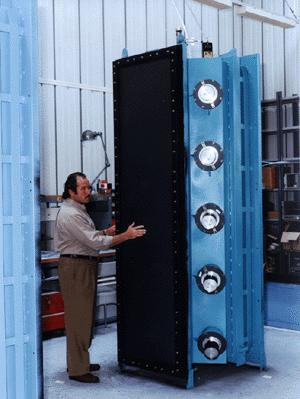
\includegraphics[angle=0,width=14cm]{gas_cer_fig1}
\caption[Gas \Cherenkov{} counter]
{Gas \Cherenkov{} counter.}
\label{fig:gas-counter}
\end{figure}
}

These two counters have identical sections but different length of 
the gas radiator, 80 cm for the left arm and 130 cm for the right arm. 
There is an additional section 50 cm long which can be attached to 
the short counter if needed.
Each \Cherenkov{} is made of 10  tubes (PMT) and 10 mirrors. 
Each mirror has a rectangular profile built in a empty sphere of interior radius 
(reflective face) of 80 cm and thickness of 1 cm. 
The very light structure of the mirror is built like honeycomb 
and is constituted as the following manner: the MgF$_2$ layer, which protect 
the aluminum; the aluminum which assure the reflectivity; 
the plexiglas, which assure a good surface; 
a sandwich (carbon-epoxy, phenolic honey comb, carbon epoxy), 
which assure the rigidity of the mirror. 

The 10 mirrors are placed just before the output window and are grouped in 
two columns of 5 mirrors. 
Each mirror reflect the light on a PMT placed at the side of the box. 
The mirrors of the same column are identical and the two columns are 
almost symmetrical. 
Positions and angles of the PMTs are not placed regularly like for the mirrors 
but were adjusted by a optical study in order to maximize the collection of light 
coming from the particular envelope of particle which have to be detected with 
the High Resolution Spectrometer (HRS) of the Hall A. 
PMT are fixed and mirrors orientation can be adjusted by hand. 

The alignment procedure use the small light source located about 820 cm
from the mirror plane in the axis of symmetry of the counter.
\infolevfour{
The picture on figs~\ref{fig:mirror-1} and~\ref{fig:mirror-6} 
shows the image of the small light source on the PMT photo-cathode during 
mirror alignment procedure. 
%
\begin{figure}[p]
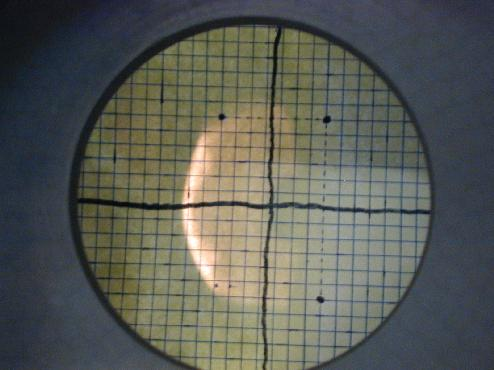
\includegraphics[angle=0,width=10cm]{gas_cer_fig3}
\caption[The image from mirror \#1 on PMT photo-cathode]
{ The image from the mirror \#1 on the PMT photo-cathode.}
\label{fig:mirror-1}
\end{figure}
%
\begin{figure}[p]
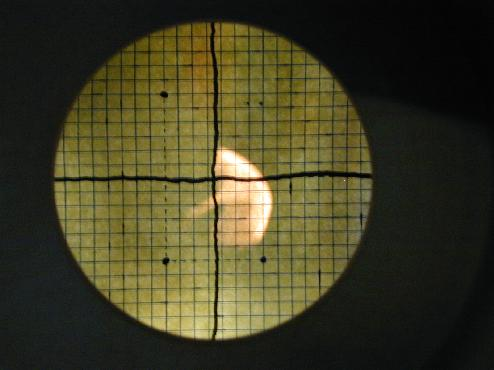
\includegraphics[angle=0,width=10cm]{gas_cer_fig2}
\caption[The image from mirror \#6 on PMT photo-cathode]
{ The image from the mirror \#6 on the PMT photo-cathode.}
\label{fig:mirror-6}
\end{figure}
}

Five photomultiplier tubes (PMT) are fixed of the two side walls. 
Each one is surrounded by a high magnetic permeability shielding (mu-metal). 
The fixing provides high voltage insulation between the PMT and the steel vessel. 
A set of optic fibers provides light pulses to each PMT for their calibration. 

\section{Safety Assessment}

\begin{safetyen}{10}{10}
The PMTs are under high voltage and care is required when handling any 
components of the counter. The body of the \Cherenkov{} counter must be grounded. 
\end{safetyen}

\section{Operating Procedure}

\paragraph{Operating Voltage}

\begin{safetyen}{10}{10}
The operating voltage on the PMTs is about -2,500 V. The voltage must be set to
zero before HV cable will be connected or disconnected from HV divider.
The HV cables must be disconnected from all HV dividers before replacement
of any PMT on the gas \Cherenkov{} counter. 
\end{safetyen}

The high voltage has to be adjusted in order to have for each PMT 
the position of the photoelectron peak at the same position 
which is around 100 channels above the pedestal. 
For good PMT the noise counting rate should not exceed 10 kHz.
Past experience show that PMT need to be replaced in average
every three years due to aging. Such short life time about 3-4 
times less than normal is due to He content in Hall A,
which led to loss of the PMT quantum efficiency.

\section{Responsible Personnel} 
The following individuals are responsible for the operation 
of the gas \Cherenkov{} counters.
 
\begin{itemize}
\item[~]Segal, John - x7242 
\item[~]Wojtsekhowski, Bogdan - x7191 
\end{itemize} 







